% Comprehensive LaTeX template
\documentclass[12pt]{article}

% --- Encoding and font packages ---
\usepackage[utf8]{inputenc} % allow UTF-8 characters
\usepackage[T1]{fontenc}    % use T1 font encoding
\usepackage{lmodern}        % improved default Latin fonts

% --- Mathematics packages ---
\usepackage{amsmath, amssymb} % enhanced math features

% --- Graphics and drawing packages ---
\usepackage{graphicx} % include external images
\usepackage{tikz}     % create drawings and diagrams
\usepackage{pgfplots} % plot data with TikZ
\pgfplotsset{compat=1.18}

% --- Color and styling ---
\usepackage{xcolor} % define and use colors

% --- Reference and hyperlink packages ---
\usepackage{hyperref}          % hyperlinks in the document
\usepackage{cleveref}          % smart cross-referencing
\usepackage{natbib}            % flexible bibliography support

% --- Units and quotations ---
\usepackage{siunitx} % consistent typesetting of units
\usepackage{csquotes} % context-aware quotes

% --- Page geometry ---
\usepackage{geometry} % easily adjust page margins
\geometry{margin=1in}

\title{Sample Document}
\author{Author Name}
\date{\today}

\begin{document}

\maketitle

\begin{abstract}
This document illustrates common LaTeX packages with explanations and simple
examples.
\end{abstract}

\section{Input and Fonts}\label{sec:fonts}
The packages \texttt{inputenc}, \texttt{fontenc}, and \texttt{lmodern} allow
typing Unicode characters and improve the default fonts.

Examples:
\begin{itemize}
  \item Accented characters can be written directly: Café, naïve, Grüß Gott.
  \item Different font styles are available, such as \textbf{bold} and
    \texttt{typewriter} text.
\end{itemize}

\section{\texttt{amsmath} and \texttt{amssymb}}\label{sec:math}
These packages extend LaTeX's math features.

Examples:
\begin{itemize}
  \item An equation:
    \begin{equation}
      E = mc^2
    \end{equation}
  \item Multiple aligned equations using special symbols:
    \begin{align}
      a^2 + b^2 &= c^2 \\
      e^{i\pi} + 1 &= 0
    \end{align}
    The set of real numbers is denoted by $\mathbb{R}$.
\end{itemize}

\section{\texttt{graphicx}}\label{sec:graphicx}
The \texttt{graphicx} package inserts images.

Examples:
\begin{figure}[h]
  \centering
  \includegraphics[width=0.3\textwidth]{example-image-a}
  \caption{A sample image.}
  \label{fig:image}
\end{figure}

\begin{figure}[h]
  \centering
  \includegraphics[width=0.3\textwidth, angle=90]{example-image-b}
  \caption{A rotated image.}
\end{figure}

\section{\texttt{tikz}}\label{sec:tikz}
TikZ creates drawings and diagrams.

Examples:

\begin{tikzpicture}
  \draw (0,0) -- (1,0) -- (1,1) -- (0,1) -- cycle;
\end{tikzpicture}

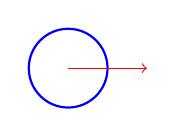
\begin{tikzpicture}
  \draw[blue, thick] (0,0) circle (0.5cm);
  \draw[->, red] (0,0) -- (1,0);
\end{tikzpicture}

\section{\texttt{pgfplots}}\label{sec:pgfplots}
The \texttt{pgfplots} package plots data.

Examples:
\begin{figure}[h]
  \centering
  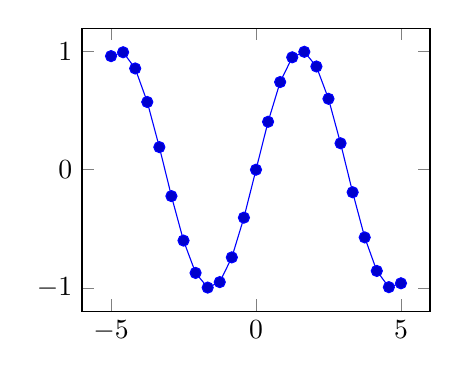
\begin{tikzpicture}
    \begin{axis}[width=6cm]
      \addplot {sin(deg(x))};
    \end{axis}
  \end{tikzpicture}
  \caption{A sine curve.}
  \label{fig:plot}
\end{figure}

\begin{figure}[h]
  \centering
  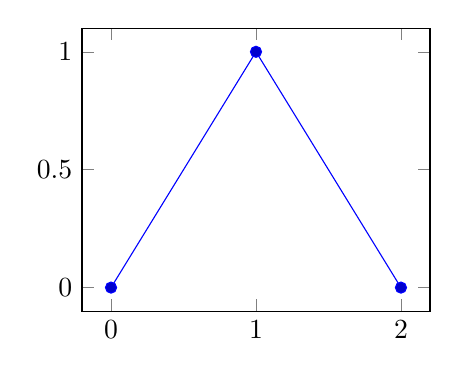
\begin{tikzpicture}
    \begin{axis}[width=6cm]
      \addplot coordinates {(0,0) (1,1) (2,0)};
    \end{axis}
  \end{tikzpicture}
  \caption{Plot from coordinates.}
\end{figure}

\section{\texttt{xcolor}}\label{sec:xcolor}
The \texttt{xcolor} package defines and uses colors.

Examples:
\begin{itemize}
  \item \textcolor{red}{This text is red.}
  \item \definecolor{mygreen}{RGB}{0,128,0}\textcolor{mygreen}{This text uses a custom green.}
\end{itemize}

\section{\texttt{hyperref}}\label{sec:hyperref}
The \texttt{hyperref} package creates hyperlinks.

Examples:
\begin{itemize}
  \item External link: \href{https://www.latex-project.org}{LaTeX Project}.
  \item Internal link: go to the \hyperref[sec:tikz]{TikZ section}.
\end{itemize}

\section{\texttt{cleveref}}\label{sec:cleveref}
The \texttt{cleveref} package simplifies cross references.

Examples:
\begin{itemize}
  \item Section reference: \cref{sec:tikz}.
  \item Figure reference: \cref{fig:plot}.
\end{itemize}

\section{\texttt{natbib}}\label{sec:natbib}
The \texttt{natbib} package handles citations.

Examples:
\begin{itemize}
  \item Textual citation: \citet{knuth1990}.
  \item Parenthetical citation: \citep{lamport1994}.
\end{itemize}

\section{\texttt{siunitx}}\label{sec:siunitx}
The \texttt{siunitx} package formats numbers and units.

Examples:
\begin{itemize}
  \item Gravitational acceleration is \SI{9.81}{\metre\per\second\squared}.
  \item A right angle is \ang{90}.
\end{itemize}

\section{\texttt{csquotes}}\label{sec:csquotes}
The \texttt{csquotes} package manages quotations.

Examples:
\begin{itemize}
  \item \enquote{Inline quotation marks are handled automatically.}
  \item \blockquote{A block quotation can span multiple lines.}
\end{itemize}

\section{\texttt{geometry}}\label{sec:geometry}
The \texttt{geometry} package sets page margins.

Examples:
\begin{itemize}
  \item This document uses one-inch margins.
  \item \newgeometry{margin=1.5in}This paragraph temporarily widens the margins.\restoregeometry
\end{itemize}

\begin{thebibliography}{9}
\bibitem[Knuth(1990)]{knuth1990} D.~E. Knuth. \emph{The TeXbook}. Addison-Wesley, 1990.
\bibitem[Lamport(1994)]{lamport1994} L. Lamport. \emph{LaTeX: A Document Preparation System}. Addison-Wesley, 1994.
\end{thebibliography}

\end{document}
